% =====================================================================
%  main.tex — WRAPPER (wiring). NIE pisz tu treści.
%  Treść jest w tresc/*.tex; wygląd w formatka/slayer.sty (bez zmian, slay-paper c2497c79).
% =====================================================================
\documentclass[11pt,a4paper]{article}

\usepackage{formatka/slayer}   % <-- FORMATKA (jedyne miejsce sterujące wyglądem)
\hypersetup{pdftitle={Slayer 150 1.01: wybór przepisu treningu przy regułach ustalanych przed każdym wynikiem}, pdfauthor={Arkadiusz Słota}, pdfcreator={SlayerLabs}, pdfproducer={SlayerLabs}}
\pdfinfoomitdate=1
\pdftrailerid{}
\pdfsuppressptexinfo=-1

\begin{document}

% =====================================================================
%  Strona tytułowa — tytuł, autor, wykres z podpisem.
% =====================================================================
\begin{titlepage}
\centering
\vspace*{1.0cm}

\slayertitle
  {Slayer 150 1.01:\\ wybór przepisu treningu przy regułach\\ ustalanych przed każdym wynikiem}%
  {Arkadiusz Słota, Fabryka AI}%
  {Wersja robocza, 7 października 2026 --- trening w toku}

\vspace{0.8cm}

\begin{figure}[h]
  \centering
  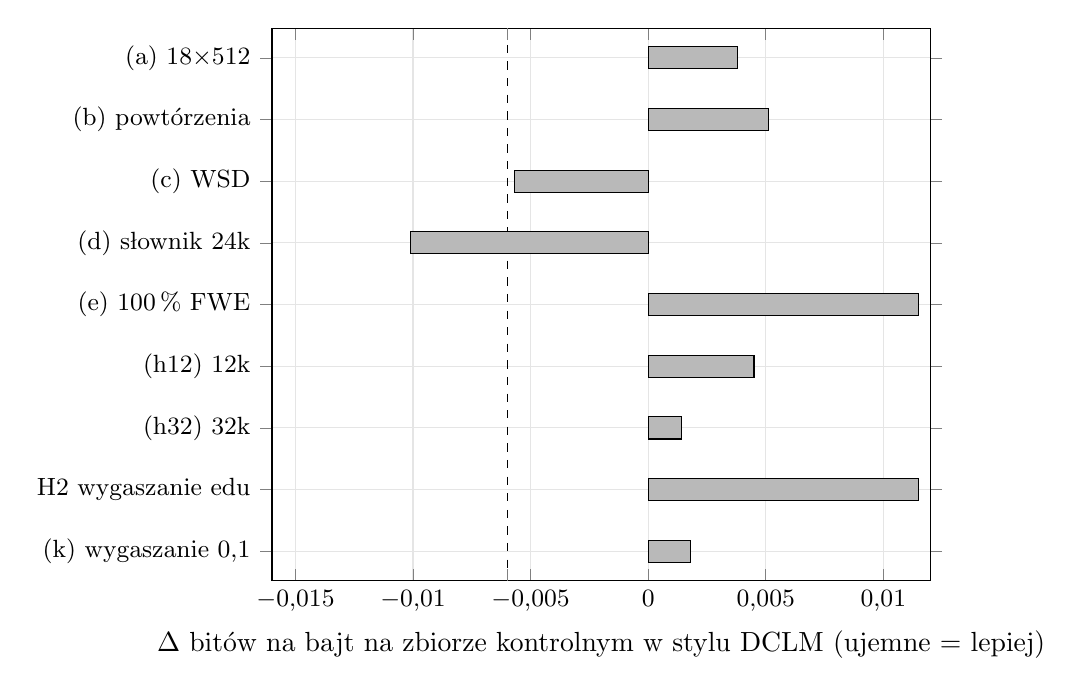
\begin{tikzpicture}
    \begin{axis}[
        xbar, width=0.82\linewidth, height=8.6cm,
        xlabel={$\Delta$ bitów na bajt na zbiorze kontrolnym w stylu DCLM (ujemne = lepiej)},
        xmin=-0.016, xmax=0.012,
        ytick={1,...,9},
        yticklabels={(a) 18$\times$512, (b) powtórzenia, (c) WSD, (d) słownik 24k, (e) 100\,\% FWE, (h12) 12k, (h32) 32k, H2 wygaszanie edu, (k) wygaszanie 0{,}1},
        scaled x ticks=false, xtick={-0.015,-0.010,-0.005,0,0.005,0.010},
        x tick label style={/pgf/number format/fixed, /pgf/number format/precision=3, /pgf/number format/use comma, font=\small},
        bar width=8pt, enlarge y limits=0.06,
        grid=major, grid style={gray!20},
        extra x ticks={-0.006}, extra x tick labels={}, extra x tick style={grid=major, grid style={black, dashed}},
        y dir=reverse, y tick label style={font=\small},
    ]
      \addplot[fill=gray!55] coordinates {
        (0.0038,1) (0.0051,2) (-0.0057,3) (-0.0101,4) (0.0115,5) (0.0045,6) (0.0014,7) (0.0115,8) (0.0018,9)};
    \end{axis}
  \end{tikzpicture}
  \caption{\textbf{Dziewięć ablacji (64M parametrów, 2 mld tokenów) ocenianych regułami zapisanymi przed każdym
  wynikiem.} Słupki pokazują zmianę liczby bitów na bajt na zbiorze kontrolnym w stylu DCLM wobec punktu
  odniesienia danego wariantu; linia przerywana to próg przyjęcia $-0{,}006$. Przekroczył go tylko słownik 24k (d).
  Słupki (e) i H2 są ucięte na $+0{,}0115$; prawdziwe wartości to $+0{,}0888$ i $+0{,}0505$. Wartości z plików
  werdyktów wymienionych w \texttt{recipe/}.}
  \label{fig:hero}
\end{figure}

\vfill
{\small Fabryka AI \textperiodcentered{} SlayerLabs \textperiodcentered{} wszystkie liczby przypięte skrótami SHA-256 do plików wyników}
\end{titlepage}
   % strona tytułowa + wykres z podpisem
% =====================================================================
%  Treść — bez preambuły.
% =====================================================================
\renewcommand{\UrlBreaks}{\do\/\do-\do\_\do.\do@}
\newcolumntype{L}[1]{>{\raggedright\arraybackslash}p{#1}}

\section*{Streszczenie}

Opisujemy, jak wybrano przepis treningu modelu Slayer 150 1.01, czyli anglojęzycznego modelu bazowego o 139,3~mln
parametrów, przygotowanego na tablicę wyników Glint Tiny-ML. Każdą zmianę przepisu najpierw sprawdzano w ablacji:
na modelu 64M trenowanym na 2~mld tokenów. Zmianę przyjmowano albo odrzucano według reguły zapisanej, zanim wynik był
znany. Każdą regułę zaimplementowano dwukrotnie, niezależnie, a obie implementacje porównano ze sobą na syntetycznych
siatkach przypadków przed użyciem. Z dziewięciu ablacji jedna została przyjęta (słownik 24k zamiast 12k), pięć
odrzucono, a trzy były nierozstrzygnięte albo pozostawiły ustawienie domyślne (rysunek~\ref{fig:hero}). Przepis
finalny to zmierzony przepis bazowy przeskalowany do 139,3~mln parametrów, ze słownikiem 24k, harmonogramem WSD
(rozgrzewka, faza stała, wygaszanie) z wygaszaniem na ostatnich 20\,\% kroków i około 24,7~mld unikalnych tokenów.
Opisujemy też problem pomiarowy samej tablicy: po ponownej ocenie czołowych modeli jedną, wspólną procedurą 11 z 12
wpisów wypada niżej niż liczby zgłoszone przez autorów, a wynik ogólny modelu z pierwszego miejsca spada z 79,67 do
76,33. Trening finalny trwa; jego wyniki zostaną dodane w kolejnej wersji.

\section{Cel i ograniczenia}

\begin{itemize}
  \item \textbf{Cel:} pierwsze miejsce na publicznej tablicy Glint Tiny-ML w wyniku ogólnym (\emph{Overall} $=$
  (BLiMP $+$ ARC-Easy $+$ WikiScore)$/3$) albo w wyniku ważonym rozmiarem modelu (\emph{eff}). Przy naszym rozmiarze
  łatwiejszy jest wynik ogólny (próg 79,67 wobec około 80,2 dla eff).
  \item \textbf{Budżet:} jedna wynajmowana karta RTX 5090 (około 1~USD za godzinę), około 55--60 godzin pracy karty na
  trening finalny.
  \item \textbf{Limit rozmiaru:} poniżej 150~mln parametrów. Model finalny ma 139\,279\,760 parametrów (współdzielona
  macierz osadzeń liczona raz).
\end{itemize}

\section{Metoda: najpierw reguła, potem wynik}

\textbf{Skala ablacji.} Wszystkie ablacje to modele 64M trenowane na 2~mld tokenów (61\,035 kroków), z tą samą
kolejnością danych. Wszystkie warianty trenowano na tej samej klasie karty (RTX 5090), a oceniano na jednej karcie
RTX 3090.

\textbf{Osie decyzyjne.} Główną miarą są bity na bajt (bpb) na dwóch zamrożonych, odłożonych zbiorach kontrolnych:
ogólnym zbiorze tekstów z sieci (w stylu DCLM) i zbiorze edukacyjnym (FineWeb-Edu, FWE). Bity na bajt nie zależą od
tokenizera, więc modele z różnymi słownikami porównujemy uczciwie. Wynik tablicy (eff) raportujemy i używamy wyłącznie
jako warunku bezpieczeństwa, bo w tej skali jest zaszumiony (odchylenie standardowe różnicy dwóch ziaren losowych
wynosi około 0,61~eff).

\textbf{Model szumu.} Szum między ziarnami losowymi szacujemy z trzech przebiegów bazowych i przyjmujemy dolną granicę
$\sigma = 0{,}002$~bpb. Aby różnica wobec średniej trzech przebiegów bazowych liczyła się jako poprawa, musi wynieść co
najmniej $-0{,}006$~bpb (około 2,1--2,6 odchylenia standardowego różnicy): na osi głównej (DCLM) dla wariantów
(a)--(d) i na obu osiach dla (e) i (h). Spadek eff nie może przekroczyć 0,56.

\textbf{Najpierw reguła.} Dla każdej ablacji regułę przyjęcia, punkt odniesienia i dane zapisywano w dzienniku decyzji
przed startem treningu. Jeśli regułę trzeba było zmienić, zmiana następowała przed jakimkolwiek wynikiem, a jej powód
był zapisywany (punkt~\ref{sec:changed}).

\textbf{Dwie implementacje.} Każdą regułę zaprogramowały dwie osoby, niezależnie od siebie. Przed każdym werdyktem
obie implementacje porównano na syntetycznych siatkach przypadków, obejmujących dokładne wartości graniczne: zgodność
360/360 dla ablacji (a)--(e), 180/180 dla (h), 48/48 dla H2 i 108/108 dla (k). Siatka dla obecnej wersji reguły
,,nie gorzej'' (g) jest w przygotowaniu. Każdy werdykt liczyły obie implementacje i musiały dać ten sam wynik.

\textbf{Kontrola powtarzalności oceny.} Zanim zaufaliśmy zmienionemu łańcuchowi oceny, ponownie oceniliśmy już
oceniony punkt kontrolny i wymagaliśmy podsumowania identycznego co do bitu (trzy takie kontrole, wszystkie
zaliczone).

\section{Ablacje (64M, 2 mld tokenów)}

Tabela~\ref{tab:ablations} podaje różnice w bpb na dwóch zbiorach kontrolnych (ujemne = lepiej) i w eff (dodatnie =
lepiej).

\begin{table}[ht]
\centering\small
\setlength{\tabcolsep}{3.5pt}\footnotesize
\begin{tabular}{@{}lL{4.4cm}rrrL{2.7cm}@{}}
\toprule
Wariant & Zmiana & $\Delta$DCLM & $\Delta$FWE & $\Delta$eff & Werdykt \\
\midrule
(a) & kształt 18$\times$512 zamiast 14$\times$576, hiperparametry bazowe & $+0{,}0038$ & $+0{,}0036$ & $-0{,}81$ & odrzucone \\
(b) & 0,755~mld unikalnych tokenów powtórzonych około 2,65 raza (ten sam budżet) & $+0{,}0051$ & $+0{,}0052$ & $-0{,}12$ & odrzucone \\
(c) & harmonogram WSD (20\,\% wygaszania) zamiast kosinusowego & $-0{,}0057$ & $-0{,}0054$ & $-0{,}24$ & nierozstrzygnięte; przyjęte jako zmiana bezkosztowa \\
(d) & słownik 24k zamiast 12k & $\mathbf{-0{,}0101}$ & $\mathbf{-0{,}0100}$ & $+0{,}61$ & \textbf{przyjęte} \\
(e) & 100\,\% FineWeb-Edu & $+0{,}0888$ & $-0{,}0161$ & $+0{,}19$ & nierozstrzygnięte (wygrywa tylko we własnej domenie) \\
(h12) & słownik 12k $+$ 2 warstwy, równa liczba parametrów, wobec (d) & $+0{,}0045$ & $+0{,}0045$ & $-1{,}33$ & odrzucone \\
(h32) & słownik 32k $-$ 1 warstwa, równa liczba parametrów, wobec (d) & $+0{,}0014$ & $+0{,}0017$ & $+0{,}34$ & odrzucone; zostaje 24k \\
H2 & wygaszanie na 100\,\% FineWeb-Edu, wobec średniej 3 kontroli & $+0{,}0505$ & $-0{,}0091$ & $+0{,}07$ & odrzucone \\
(k) 0,1 & wygaszanie 10\,\% wobec 20\,\% & $+0{,}0018$ & $+0{,}0020$ & $-0{,}38$ & zostaje 20\,\% \\
(k) 0,3 & wygaszanie 30\,\% wobec 20\,\% & $-0{,}00001$ & $-0{,}0002$ & $+0{,}12$ & zostaje 20\,\% \\
\bottomrule
\end{tabular}
\caption{Werdykty ablacji. Każdą regułę zapisano przed treningiem; każdy werdykt policzyły dwie niezależne
implementacje.}
\label{tab:ablations}
\end{table}

Zakres wniosków:
\begin{itemize}
  \item \textbf{(a)} odrzuca kształt 18$\times$512 \emph{przy bazowym współczynniku uczenia i rozgrzewce}, a nie
  głębokość w ogóle.
  \item \textbf{(d)} porównuje równe liczby tokenów, a nie bajtów. W naszej puli danych token słownika 24k niesie o
  około 9,0\,\% więcej tekstu niż token 12k (ta sama pula to 9,39~mld tokenów w 12k i 8,62~mld w 24k), więc część
  zysku to ,,więcej tekstu za ten sam budżet tokenów''. \textbf{(h)} usuwa wpływ liczby parametrów: przy równej liczbie
  parametrów słownik 12k z większą liczbą warstw wypada gorzej, a 32k z mniejszą liczbą warstw nie wypada lepiej.
  \item \textbf{(h32)} ma nieco wyższy wynik tablicy ($+0{,}34$~eff, $+0{,}97$ ARC-Easy), ale gorsze bpb na obu osiach.
  Obie różnice mieszczą się w szumie; rozstrzygnęła reguła zapisana przed treningiem, oparta na bpb.
  \item \textbf{H2} sprawdzało, czy kończenie treningu na tekstach edukacyjnych pomaga w tablicy. Przesuwa model w
  stronę BLiMP i FineWeb-Edu, pogarsza ogólny tekst z sieci i Wikipedię (perpleksja bajtowa $+0{,}095$) i nie zmienia
  wyniku tablicy. Przebiegi kontrolne H2 zmierzyły też szum samej fazy wygaszania: $\sigma_{\mathrm{par}} =
  0{,}00028$~bpb (DCLM), czyli około czterokrotnie mniej niż szum między ziarnami.
\end{itemize}

\section{Przepis finalny}

\begin{table}[ht]
\centering\small
\begin{tabular}{@{}L{3.2cm}L{11.0cm}@{}}
\toprule
Ustawienie & Wartość \\
\midrule
Kształt & 17 warstw $\times$ 768, 12 głów uwagi (proporcje bazowe przeskalowane) \\
Słownik & 24\,576 tokenów, bajtowy BPE wytrenowany na naszej puli; 4,02 bajta na token na odłożonym tekście angielskim; bezstratne odtworzenie tekstu \\
Parametry & 139\,279\,760 (osadzenia 18,9~mln) \\
Trener & trener referencyjny na jedną kartę; Muon dla wag dwuwymiarowych, AdamW dla pozostałych \\
Partia, kontekst & 32 $\times$ 1024 tokeny na krok \\
Harmonogram & WSD, wygaszanie na ostatnich 20\,\% kroków \\
Tokeny & około 24,7~mld (754\,453 kroki; trening skrócony do liczby dostępnych unikalnych tokenów), bez dodatkowych epok; wewnętrzne powtórzenia samej puli (kopie dokumentów związanych z ARC, 12,0\,\% puli, i OpenStax $\times$4, 1,5\,\%) są częścią zmierzonego przepisu \\
Dane & zmierzona mieszanka bazowa (8,6~mld tokenów) dopełniona z tych samych źródeł w przybliżeniu w tych samych proporcjach (krótsze źródła rozłożone na pozostałe; praca towarzysząca) \\
Kolejność danych & stała kolejka slotów z zapisanymi skrótami SHA-256; wznawianie tylko na granicach slotów \\
\bottomrule
\end{tabular}
\caption{Przepis treningu finalnego.}
\label{tab:recipe}
\end{table}

\textbf{Dlaczego nie stroiliśmy mieszanki.} Ablacja (e) pokazała, że zmiana udziału tekstów edukacyjnych daje duże
efekty, różne na różnych osiach, więc nie ekstrapolowaliśmy nowej mieszanki z dwóch punktów. Dopełnienie zachowuje
proporcje bazowe. Zanim dopełnione dane wejdą do treningu, muszą przejść zapisany z góry \textbf{test ,,nie gorzej''
(g)}: model 64M trenowany na losowej próbce 2~mld tokenów \emph{dokładnie tej} mieszanki finalnej nie może być gorszy
od modelu kontrolnego ze słownikiem 24k o więcej niż $+0{,}006$~bpb na żadnej z osi ani o więcej niż $0{,}99$~eff.
Jeśli test nie przejdzie albo się spóźni, trening kończy się na samej puli bazowej (plan B), z wygaszaniem na tej
puli. Moment przełączenia ustalamy z góry razem z mieszanką, więc test zawsze mierzy dokładnie tę mieszankę, którą
zobaczy trening.

\textbf{Mieszanie na poziomie dokumentów.} W chwili wejścia dopełnienia niewykorzystana część puli bazowej i nowe dane
są mieszane w jednej permutacji całych dokumentów. Faza wygaszania widzi więc tę samą mieszankę, którą zmierzył test
(g), a nie naprzemienne bloki starych i nowych danych.

\textbf{Długość treningu wynika z danych.} Dopełnienie daje 4,09 bajta na token zamiast planowanych 4,0, więc trening
skrócono do liczby dostępnych unikalnych tokenów (około 24,7~mld, 754\,453 kroki zamiast 762\,940), zamiast powtarzać dane; wygaszanie zachowuje udział
20\,\% nowej długości.

\section{Fakty inżynierskie, od których zależy przepis}

\begin{itemize}
  \item \textbf{Przepustowość} na jednej karcie RTX 5090 przy partii 32 (ta sama sonda dla wszystkich kształtów):
  108,6~mln $\to$ 156\,720 tokenów/s; 122,8~mln $\to$ 136\,250; 144,0~mln (12k) $\to$ 117\,290; \textbf{139,3~mln (24k)
  $\to$ 124\,798}. Przy tej wielkości kształt 24k (139,3~mln) jest o 6,4\,\% szybszy niż kształt 12k (144,0~mln).
  Trwający trening finalny utrzymuje 117--121 tys. tokenów/s; powolny spadek wynika z limitu mocy karty.
  \item \textbf{Wznowienie jest dokładne na tej samej klasie karty.} Wznowienie fazy wygaszania z punktu kontrolnego na
  innej karcie RTX 5090 odtworzyło pierwotny przebieg z dokładnością $3\cdot10^{-7}$~bpb (DCLM) i $4\cdot10^{-6}$~bpb
  (FineWeb-Edu). Przejście na trening na wielu kartach poprzedza test równoważności z progami ustalonymi z góry.
  \item \textbf{Tożsamość danych sprawdzamy skrótami, a nie opisem procedury.} Każde odtworzenie puli na nowej
  maszynie dało ten sam plik co do bitu. Tokenizacja dopełnienia dała identyczne bajty na dwóch różnych maszynach i
  systemach operacyjnych na pliku testowym; tożsamość całego zmieszanego regionu jest sprawdzana skrótem przed użyciem.
  \item \textbf{Dekontaminacja} dopełnienia względem WikiText-2, ARC (zbiory testowe i walidacyjne) i BLiMP oraz
  usunięcie nakładania z naszymi zbiorami kontrolnymi usunęły 25\,808 z 11,4~mln dokumentów (praca towarzysząca).
\end{itemize}

\section{Co poszło nie tak i co poprawiliśmy przed wynikami}
\label{sec:changed}

\begin{itemize}
  \item Pierwszy margines bezpieczeństwa dla eff w teście ,,nie gorzej'' ($-0{,}495$) wynosił jedno odchylenie
  standardowe, przez co dobra mieszanka byłaby odrzucana w około 16\,\% przypadków. Przed jakimkolwiek wynikiem (g)
  poszerzyliśmy go do $-0{,}99$.
  \item Pierwsza reguła H2 opierała się na jednej, zaszumionej parze przebiegów; symulacja pokazała do 8,6\,\%
  fałszywych przyjęć. Przed pierwszym przebiegiem H2 zastąpiliśmy ją regułą z trzema przebiegami kontrolnymi i
  dokładnie 5\,\% fałszywych przyjęć.
  \item Pierwsza propozycja reguły (k) miała jeden warunek: $\Delta\mathrm{DCLM} \le -0{,}002$ (jedno $\sigma$ między
  ziarnami). Wobec znanego wtedy szumu to około 0,7 odchylenia standardowego różnicy dwóch przebiegów, czyli w
  przybliżeniu normalnym około 24\,\% fałszywych zmian na wariant. Przed (k) przebudowaliśmy regułę:
  $\Delta\mathrm{DCLM} \le -\max(0{,}002;\ t\,\sigma_{\mathrm{par}}\sqrt{2})$, gdzie $\sigma_{\mathrm{par}}$ zmierzono
  na fazie wygaszania, plus $\Delta\mathrm{FWE} \le 0$ i warunek bezpieczeństwa dla eff. Zmierzony szum wygaszania
  ($\sigma_{\mathrm{par}} = 0{,}00028$) okazał się mały, więc wiąże dolna granica 0,002, a próg to około pięciu
  odchyleń standardowych różnicy dwóch wygaszeń.
  \item Test ,,nie gorzej'' (g) pierwotnie porównywał wynik z przebiegami bazowymi ze słownikiem 12k; wtedy zysk ze
  słownika przepuściłby dowolną mieszankę. Przed testem zmieniliśmy punkt odniesienia na model ze słownikiem 24k.
\end{itemize}

\section{Problem pomiarowy tablicy wyników}

Tablica podaje liczby zgłoszone przez autorów, z których każda została zmierzona ich własną procedurą oceny. Przy
jednej, wspólnej procedurze (dodatek~\ref{app:protocol}) nasza ponowna ocena czołowych wpisów daje
tabelę~\ref{tab:board}.

\begin{table}[ht]
\centering\small
\begin{tabular}{@{}lrL{6.2cm}@{}}
\toprule
Model & Zgłoszony wynik ogólny & Wynik ogólny po ponownej ocenie (wspólna procedura) \\
\midrule
Haidass-143M & 79,67 & 76,33 (ARC-Easy 56,23 wobec zgłoszonych 60,23) \\
GPT-X2-125M & 79,45 & 77,67 \\
GoLLeM-v5 128M (nasz) & --- & 76,30 \\
\bottomrule
\end{tabular}
\caption{Zgłoszony i ponownie oceniony wynik ogólny czołowych wpisów.}
\label{tab:board}
\end{table}

Przy wspólnej procedurze 11 z 12 ponownie ocenionych wpisów wypada niżej niż zgłoszone liczby, a kolejność się
zmienia: pierwsze miejsce ma GPT-X2 z wynikiem 77,67, a nasz poprzedni model traci do Haidass 0,03 punktu. Najbardziej
prawdopodobnym wyjaśnieniem są różnice między procedurami oceny (format promptu, normalizacja, ustawienia few-shot);
nie twierdzimy, że którakolwiek zgłoszona liczba jest błędna w ramach własnej procedury. Wielkość tego efektu zależy
też od modelu (nasz v5 zyskuje $+1{,}05$ w lm-eval 0.4.13, inny model $+2{,}61$), więc liczb z różnych procedur nie da
się przeliczyć stałą. Model finalny przedstawimy w obu wersjach: w lm-eval 0.4.13 na wersjach zbiorów ustalonych przez
ewaluator Fabryka track oraz we wspólnej procedurze, obok ponownie ocenionych wpisów.

\section{Stan prac i ograniczenia}

\begin{itemize}
  \item Trening finalny trwa. Żaden jego punkt kontrolny nie jest podstawą decyzji poza twardymi awariami (NaN, skoki
  straty, gwałtowny wzrost normy gradientu), a żadnego wyniku pośredniego nie porównujemy z progiem tablicy. Ze względu
  na zmianę dostawcy mocy obliczeniowej trening zostanie wznowiony od ustalonego punktu kontrolnego na granicy slotu
  na nowej maszynie; dopełnienie (jeśli test (g) przejdzie) wchodzi w tym samym punkcie.
  \item Wszystkie ablacje mają 64M parametrów i 2~mld tokenów; model finalny ma 139M parametrów i około 24,7~mld tokenów.
  Kierunki efektów przenoszą się pewniej niż ich wielkości.
  \item Jedno ziarno losowe na wariant ablacji ($n = 1$), z odpowiednio dobranymi progami.
  \item Gotowego tokenizera 49k (SmolLM2) jeszcze nie porównaliśmy; test jest zaprojektowany (dwa warianty, które
  obejmują skalę docelową z obu stron) i jego wynik podamy w kolejnej wersji.
\end{itemize}

\appendix
\section{Wspólna procedura oceny}
\label{app:protocol}

\begin{itemize}
  \item \textbf{Wynik:} Overall $=$ (dokładność BLiMP $+$ dokładność ARC-Easy $+$ WikiScore)$/3$, gdzie WikiScore
  przekształca perpleksję bajtową na WikiText-2 na skalę 0--100 w skali logarytmicznej, tak jak na tablicy.
  \item \textbf{Zbiory (ustalone wersje):} \path{EleutherAI/wikitext_document_level} @6472347,
  \path{nyu-mll/blimp} @877fba0, \path{allenai/ai2_arc} (ARC-Easy, test) @210d026.
  \item \textbf{Ocena ARC-Easy:} logarytm prawdopodobieństwa odpowiedzi przy danym pytaniu, bez normalizacji długości
  (\texttt{acc}), tak jak na tablicy.
  \item \textbf{Narzędzia:} nasz wspólny kod oceny oraz lm-eval 0.4.13 dla liczb w formacie tablicy. Skróty skryptów
  i pliki wyników dla każdego modelu są wymienione w katalogu \texttt{recipe/} tego wydania.
\end{itemize}
             % właściwa treść (body)

\end{document}
